%! TeX program = lualatex
\documentclass[twoside, a4paper, 12pt]{book}

\title{Geometryczna Teoria Grup}
\author{\color{subtext1}Weronika Jakimowicz}
\date{Zima 2024/25}

% \usepackage[utf8]{inputenc}
\usepackage[T1]{fontenc}

\usepackage{fontspec}

\usepackage[default]{cantarell}


\usepackage[
  a4paper,
  total={170mm, 247mm},
  left=20mm,
  top=25mm,
  % showframe
]{geometry}

\usepackage[skip=3mm]{parskip}
\renewcommand{\baselinestretch}{1.2}
\selectfont


\usepackage{amsfonts}
\usepackage{amsmath}
\usepackage{amssymb}

\usepackage{mathastext}

\DeclareMathOperator{\Spec}{Spec}

\usepackage{xcolor}

\definecolor{rosewater}{HTML}{dc8a78}
\definecolor{flamingo}{HTML}{dd7878}
\definecolor{pink}{HTML}{ea76cb}
\definecolor{mauve}{HTML}{8839ef}
\definecolor{red}{HTML}{d20f39}
\definecolor{maroon}{HTML}{e64553}
\definecolor{peach}{HTML}{fe640b}
\definecolor{yellow}{HTML}{df8e1d}
\definecolor{green}{HTML}{40a02b}
\definecolor{teal}{HTML}{179299}
\definecolor{sky}{HTML}{04a5e5}
\definecolor{sapphire}{HTML}{209fb5}
\definecolor{blue}{HTML}{1e66f5}
\definecolor{lavender}{HTML}{7287fd}
\definecolor{subtext2}{HTML}{4c4f69}
\definecolor{subtext1}{HTML}{5c5f77}
\definecolor{subtext0}{HTML}{6c6f85}
\definecolor{overlay2}{HTML}{7c7f93}
\definecolor{overlay1}{HTML}{8c8fa1}
\definecolor{overlay0}{HTML}{9ca0b0}

\definecolor{text}{HTML}{000000}
\color{text}

\makeatletter 
\let\htitle\@title
\let\fauthor\@author
\makeatother

\usepackage{fancyhdr}

\fancyfoot[CE, CO]{}
\fancyfoot[LE, RO]{\color{overlay2}\thepage}

\fancyhead[RE, LO]{$ \quad $\color{subtext1}\fauthor $ \quad $}
\fancyhead[LE, RO]{$ \quad $\color{green!40!subtext2}\bfseries\htitle $ \quad $}

\fancypagestyle{plain}{%
  \fancyhf{}%
  \fancyfoot[CE, CO]{}
  \fancyfoot[LE, RO]{\color{overlay2}\thepage}

  \fancyhead[RE, LO]{$ \quad $\color{subtext1}\fauthor $ \quad $}
  \fancyhead[LE, RO]{$ \quad $\color{green!40!subtext2}\bfseries\htitle $ \quad $}
}
\usepackage{dashrule}

\renewcommand{\headrule}{\color{overlay0}\hdashrule[.5ex]{\headwidth}{1pt}{1pt}}

\pagestyle{fancy}

\usepackage{titlesec}

\titleformat{\chapter}[block]{\bfseries\Huge}{\color{green!40!subtext2}\filright\Huge\thechapter.}{1ex}{\color{green!40!subtext2}\Huge\filright}

\titlespacing*{\chapter}{0pt}{0pt}{20pt}

\usepackage{amsthm}
\usepackage{thmtools}
\usepackage{tcolorbox}

% \RequirePackage[framemethod=TikZ]{mdframed}

\tcbuselibrary{theorems}
\tcbuselibrary{breakable}
\tcbuselibrary{skins}

\tcbset{greenTHM/.style={
    fonttitle = \bfseries\large,
    coltitle = green!50!black,
    description color = green!50!black, 
    description font = \bfseries\large,
    colbacktitle = white, %green!40!black!75,
    breakable, 
    enhanced,
    attach boxed title to top left = {
      xshift=0.5cm, 
      yshift=-\tcboxedtitleheight/2
    },
    boxed title style = {
      boxrule=0pt,
      colframe=white
    },
    top=6mm,
    bottom=4mm,
    colback=white,
    frame hidden,
    borderline={1pt}{0pt}{green!40},
    arc=0mm,
    after skip=5mm,
    before skip=5mm
  }
}

\tcbset{orangeTHM/.style={
    fonttitle = \bfseries\large,
    coltitle = orange!60!black,
    description color = orange!60!black, 
    description font = \bfseries\large,
    colbacktitle = white, %green!40!black!75,
    breakable, 
    enhanced,
    attach boxed title to top left = {
      xshift=0.5cm, 
      yshift=-\tcboxedtitleheight/2
    },
    boxed title style = {
      boxrule=0pt,
      colframe=white
    },
    top=6mm,
    bottom=4mm,
    colback=white,
    frame hidden,
    borderline={1pt}{0pt}{orange!40}, 
    arc=0mm,
    before skip=5mm,
    after skip=5mm
  }
}

\NewTcbTheorem[
  auto counter, 
  % number within=chapter
  number within=section
]{definition}{Definition}{greenTHM}{def} 

\NewTcbTheorem[
  use counter from=definition
]{theorem}{Theorem}{orangeTHM}{th}

\NewTcbTheorem[
  use counter from=definition
]{proposition}{Proposition}{orangeTHM}{prop}


\usepackage{svg}

\renewenvironment{proof}{{\bfseries\color{green!60!black} Dowód}$ $\newline}{
  \begin{flushright} \includesvg[width=4mm]{../../../../duck.svg} \end{flushright}$ $\newline
}

\usepackage{soul}

\sethlcolor{green!15}

\makeatletter
%\font\SOUL@tt="LMMono10-Regular"
\setbox\z@\hbox{\SOUL@tt-}
\SOUL@ttwidth\wd\z@ %
\makeatother

\newcommand{\buff}[1]{
  {\bfseries\color{green}#1}
}

\usepackage{enumitem}

\usepackage[dates, pl]{../../../template}

\usepackage{halloweenmath}

\begin{document}
\frontmatter 
\maketitle
\thispagestyle{empty}
\setcounter{page}{0}

\tableofcontents
\mainmatter

\pagestyle{fancy}
  
\section{02.10.2024}{Grafy Cayleya}

\subsection{Metryka słów}

\begin{definition}{metryka słów}{}
  Niech $G$ będzie grupą, a $S$ dowolnym układem jej generatorów. Wówczas dla dowolnych $g_1,g_2\in G$ \buff{odległość między nimi w metryce słów} definiujemy jako
$$ds(g_1, g_2)=\min\{n\;:\;g_2=g_1s_1,...,s_n,\;s_i\in S\cup S^{-1}\},$$
gdzie $S^{-1}=\{g^{-1}\;:\;g\in S\}$.
\end{definition}

Metryka słów jest 
\begin{enumerate}
  \item skończona
  \item symetryczna (z definicji generatorów)
  \item \hl{lewo-niezmiennicza}, czyli $(\forall\;\gamma\in G)\;ds(\gamma g_1,\gamma g_2)=ds(g_1, g_2)$
\end{enumerate}
Ostatnia własność oznacza, że $G$ działa na sobie jako na przestrzeni metrycznej przez izometrie.

Gromov chce patrzeć na dyskretne przestrzenie metryczne, jakimi są grupy z metryką słów, jako na przestrzenie ciągłe (z dużej odległości).

\subsection{Graf Cayleya}

\begin{definition}{graf Cayleya}{}
Niech $G$ będzie grupą, a $S$ zbiorem jej generatorów. $C(G, S)$ to graf Cayleya o wierzchołkach będących elementami $G$ i skierowanych krawędziach etykietowanych generatorami:
\begin{center}
  \begin{tikzcd}
    g\arrow["s", r] & gs
  \end{tikzcd}
\end{center}
gdzie $g\in G$ i $s\in S$.
\end{definition}

\begin{example}[m]
\item Dla $G=\Z^2$ oraz $S=\{{\color{red}\overbrace{(1, 0)}^s}, {\color{blue}\overbrace{(0, 1)}^t}\}$ graf Cayleya to nieskończona "kratka"
  \bigskip

  \begin{center}
    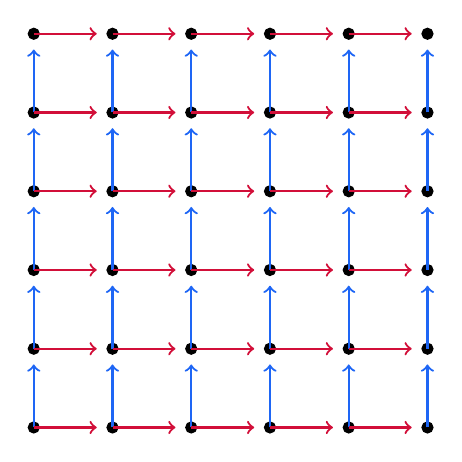
\begin{tikzpicture}
      \foreach \x in{0,...,5} { 
        \foreach \y in{0,...,5} {
          \filldraw (\x, \y) circle (2pt);
        }
      }

      \foreach \x in {0,...,5} {
        \foreach \y in {0,..., 4} {
          \draw[->, blue, thick] (\x, \y) -- (\x, \y+.8);
        }
      }
      \foreach \x in {0,...,4} {
        \foreach \y in {0,..., 5} {
          \draw[->, red, thick] (\x, \y) -- (\x+.8, \y);
        }
      }
    \end{tikzpicture}
  \end{center}
\item Dla grupy cyklicznej rzędu $p$ z generatorem $\color{red}s$ graf Cayleya to $p$-kąt
  \begin{center}
    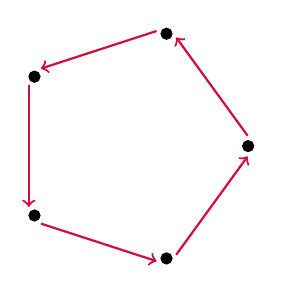
\begin{tikzpicture}
      \foreach \i in {0,..., 4} {
        \filldraw ( 360 /5 * \i :1.5) circle (2pt);
        \draw[->, red, thick] (360/5*\i + 5:1.5) -- (360/5*\i + 360/5 - 5:1.5);
      }
    \end{tikzpicture}
  \end{center}
\item {\color{red}\Large TO DO} parkietarz kwadratami
\end{example}

Każdy graf Cayleya jest \buff{spójny}, bo jego krawędzie to mnożenie przez generatory. Dodatkowo, grupa $G$ działa na nim przez \hl{automorfizmy zachowując krawędzie oraz ich etykiety}. To znaczy, że krawędż z wierzchołkami \begin{tikzcd}g\arrow[r, "s"]&gs\end{tikzcd} pod działaniem elementu $\gamma \in G$ staje się \begin{tikzcd}\gamma g\arrow[r, "s"] & \gamma gs\end{tikzcd}.

Jeśli każdą krawędź w grafie Cayleya potraktujemy jako odcinek długości $1$, to możemy na nim zdefiniować metrykę która jako odległość dwóch punktów przyjmuje długość najkrótszej ścieżki między nimi. Ta metryka na wierzchołkach pokrywa się z \buff{metryką słów} na grupie $G$ o generatorach $S$, której graf rozpatrujemy. Przy takiej metryce działanie grupy $G$ jest więc działaniem nie tylko przez automorfizmy, ale przez izometrie (lewa-niezmienniczość).

%
% \section{25.02.2025}{Produkty i koprodukty kategorii}

\subsection{O obiektach początkowych i końcowych słów kilka}

\begin{definition}{obiekt początkowy i końcowy}{}
  Powiemy, że obiekt $C\in \Cc_0$ jest \buff{początkowy}, jeśli dla każdego $D\in\Cc_0$ istnieje dokładnie jeden morfizm $C\to D$, $|\Cc(C, D)|=1$. Analogicznie definiujemy \buff{obiekt końcowy} $C$: $\forall\;D\in\Cc_0\;|\Cc(D, C)|=1$.
\end{definition}

\begin{example}[m]
  \item W kategorii, której obiektami jest odcinek $\Cc_0=[0,1]$, a morfizmy to relacja $\leq$ obiektem początkowym jest $0$, a końcowym - $1$.
  \item W kategorii zbiorów obiektem początkowym jest $\emptyset$, a obiektem końcowym jest singleton.
  \item W $Gr$ grupa trywialna jest zarówno obiektem początkowym jak i końcowym.
  \item Kategoria, która ma dwa obiekty bez morfizmów między nimi nie ma obiektu końcowego ani początkowego.
\end{example}

\begin{fact}{}{}
  Obiekty końcowe i początkowe, jeśli istnieją, to są jedyne z dokładnością do izomorfizmu.
\end{fact}

\begin{proof}
  Niech $C$ i $C'$ będą obiektami końcowymi kategorii $\Cc$. Wiemy, że $\Cc(C, C)=\{id_C\}$, czyli komutujący diagram
  \begin{center}
    \begin{tikzcd}
      C \arrow[rr, "id_C"]\arrow[dr, "\exists!f" below left] & & C\\ 
                           & C'\arrow[ur, "\exists!g" below right]
    \end{tikzcd}
  \end{center}
  daje $g\circ f=id_C$. Analogiczny diagram daje $f\circ g=id_{C'}$. Stąd $f$ i $g$ to para wzajemnie odwrotnych izomorfizmów między $C$ i $C'$
\end{proof}

\subsection{(Ko)granice funktorów a (ko)produtky}

Niech $F:\mathcal{I}\to \Cc$ będzie funktorem, gdzie o kategorii $\mathcal{I}$ myślimy jako o kategorii indeksów. Przez $\Cc^{\mathcal{I}}$ oznaczmy kategorię wszystkich takich funktorów. 
Powiemy, że funktor $C$ jest stały, jeżeli $C(i)=C$ dla każdego $i\in\mathcal{I}_0$ oraz $C(f)=id_C$ dla każdego morfizmu.

Budujemy kategorię, której 
\begin{itemize}
  \item obiekty to wszystkie naturalne przekształcenia funktora $F$ w funktory stałe $C$, $\phi:F\implies C$, czyli komutujące diagramy (kostożki) 
    \begin{center}
      \begin{tikzcd}
        F(i)\arrow[rr, "F(f)"]\arrow[dr, "\phi_i" below left] & & F(j)\arrow[dl, "\phi_j"]\\ 
                                                  & C
      \end{tikzcd}
    \end{center}
  \item a morfizmy to strzałki $C\to D$ takie, że diagram
    \begin{center}
      \begin{tikzcd}
        C\arrow[rr] & & D\\ 
                    & F\arrow[ur, Rightarrow, blue, "\phi" below right]\arrow[ul, Rightarrow, orange, "\psi" below left]
      \end{tikzcd}
    \end{center}
    komutuje.
\end{itemize}

Diagram wyżej można rozpisać jako:
\begin{center}
  \begin{tikzcd}[column sep=large]
    & F(i)\arrow[d] \arrow[ddl, "\phi_i" above left, blue]\arrow[ddr, "\psi_i" above right, orange] \\ 
    & F(j)\arrow[dl, "\phi_j" above, blue]\arrow[dr, "\psi_j" above, orange]\\ 
    D & & C\arrow[ll]
  \end{tikzcd}
\end{center}

\begin{definition}{kogranica funktora}{}
  \buff{Kogranicą} (\acc{granica prosta}) funktora $F$, $\varinjlim F$, nazywamy obiekt początkowy w wyżej zdefiniowanej kategorii naturalnych przekształceń. 
  % \buff{Granica} (\acc{granica odwrotna}) to wtedy obiekt końcowy powyższej kategorii ze wszystkimi strzałkami zdualizowanymi $\varprojlim F$.
\end{definition}

Diagram wyżej możemy zdualizować i zamiast rozpatrywać naturalne przekształcenia $\phi:F\implies C$ możemy rozważyć naturalne przekształcenia $\phi:C\implies F$, czyli diagramy (stożki)
\begin{center}
  \begin{tikzcd}
    & C \arrow[dl, "\phi_i" above left] \arrow[dr, "\phi_j" above right]\\ 
    F(i)\arrow[rr, "F(f)" below] & & F(j)
  \end{tikzcd}
\end{center}
z morfizmami {definiowanymi analogicznie. 

\begin{definition}{granica funktora}{}
  \buff{Granica} (\acc{granica odwrotna}) to obiekt końcowy powyższej kategorii stożków, $\varprojlim F$.
\end{definition}

% {\color{red}tutaj jest zdjecie
%
% przyklad dla kategorii zbiorów
%
% ja chyba chce wziąć dwuelementową kategorię $\mathcal{I}$ i tutaj policzyć, jeśli $F(1)=G$, a $F(2)=H$.
% }
%
Rozważmy kategorię $\mathcal{I}$, która ma dwa obiekty $\mathcal{I}_0=\{0,1\}$. Niech $F:\mathcal{I}\to Set$ będzie funktorem, dla którego $F(0)=A$, a $F(1)=B$. Niech $\phi$ oraz $\psi$ będzie parą naturalnych przekształceń, dla których
\begin{center}
  \begin{tikzcd}[column sep=large, row sep=large]
     & \varinjlim F\arrow[dl, "\phi_0" above left] \arrow[dr, "\phi_1"] \\ 
    F(0)=A & D \arrow[l, "\psi_0"] \arrow[r, "\psi_1" below right] \arrow[u, "\exists!f", dashed] & F(1)=B
  \end{tikzcd}
\end{center}
gdzie pionowa strzałka istnieje i jest jedyna, bo $\varinjlim F$ to obiekt końcowy. Jeśli weźmiemy $\varinjlim F=A\times B$, a $\phi_0=\pi_A$ oraz $\phi_1=\pi_B$ będą rzutami i $f(d)=(\psi_0(d), \phi_1(d))$, to diagram nadal jest prawdziwy. 

Granica odwrotna tego samego funktora, to z kolei suma rozłączna $A\sqcup B$, bo diagram
\begin{center}
  \begin{tikzcd}[column sep=large, row sep=large]
    F(0)=A\arrow[r, "\psi_0"]\arrow[dr, "\phi_0=i_A" below left] & D & F(1)=B\arrow[l, "\psi_1" above]\arrow[dl, "\phi_1=i_B"]\\ 
                                                       & \varprojlim F= A\sqcup B \arrow[u, dashed, "\exists!f"]
  \end{tikzcd}
\end{center}
gdzie $f(x)=\phi_0(x),$ jeśli $x\in A$ oraz $f(x)=\psi_1(x)$ jeśli $x\in B$, komutuje.

\begin{definition}{(ko)produkt}{}
  \buff{Produktem} obiektów $A$ i $B$ kategorii $\Cc$ nazywamy granicę prostą (kogranicę) funktora $F:\mathcal{I}\to \Cc$ dla $\mathcal{I}$ oraz $F$ jak wyżej.

  \buff{Koproduktem} obiektów $A$ i $B$ kategorii $\Cc$ nazywamy granicę odwrotną (granicę) funktora $F:\mathcal{I}\to\Cc$
\end{definition}

\begin{example}[m]
  \item W kategorii grup produkt to iloczyn kartezjański dwóch grup, tak jak w kategorii zbiorów, tj. dla grup $A,G,H$ komutuje diagram
    \begin{center}
      \begin{tikzcd}[column sep=large, row sep=large]
        & G\times H\arrow[dl, "\pi_G" above left]\arrow[dr, "\pi_H"]\\ 
        G & A\arrow[l, "g"]\arrow[r, "h"]\arrow[u, "g\times h" below] & H
      \end{tikzcd}
    \end{center}
    Koprodukt to z kolei produkt wolny tych dwóch grup:
\begin{center}
  \begin{tikzcd}[column sep=large, row sep=large]
    G\arrow[r, "g"]\arrow[dr, "i_G" below left] & A & H\arrow[l, "h" above]\arrow[dl, "i_H"]\\ 
                                                       & H\ast G \arrow[u, dashed, "\exists!f"]
  \end{tikzcd}
\end{center}
gdzie $f$ nakłada na litery słów $G\ast H$ pochodzące z $G$ morfizm $g$, a na litery pochodzące z $H$ - morfizm $h$.
  \item Niech $F:\mathcal{I}\to (P, \leq)$ z dwuobiektowej kategorii $\mathcal{I}$ w zbiór uporządkowany. Wtedy jeśli mamy diagram 
    \begin{center}
      \begin{tikzcd}
         & \varinjlim F\arrow[dr]\arrow[dl] \\ 
        F(0)=a & d \arrow[l]\arrow[r]\arrow[dashed, u] & F(1)=b
      \end{tikzcd}
    \end{center}
    to znaczy, że $d\leq a$, $d\leq b$ oraz $d\leq \varinjlim{F}$. Żeby więc miało to sens dla dowolnego $d\leq a,b$ to $\varinjlim F=\inf\{a,b\}$. Analogicznie dostajemy, że $\varprojlim F=\sup\{a,b\}$.

  \item Jeśli $\mathcal{I}$ jest kategorią o nieskończenie wielu obiektach bez morfizmów między różnymi obiektami, a $F:\mathcal{I}\to Set$ jest funktorem w kategorię zbiorów, to wówczas kogranicą tego funktora jest nieskończony iloczyn kartezjański $\prod_{i\in\mathcal{I}_0}F(i)$, a granicą - nieskończona suma rozłączna $\bigsqcup_{i\in\mathcal{I}_0}F(i)$.
\end{example}

% kategoria nieskończenie wiele elementów, ale bez strzałek (jako $\mathcal{I}$)
 % Niech $C$ oraz $C'$ będą kogranicami tego samego funktora. Z definicji mamy
% \begin{center}
%   \begin{tikzcd}[column sep=large, row sep=large]
%     & F(i)\arrow[dr, "\phi_i"]\arrow[d, "\psi_i"]\arrow[dl, "\phi_i" above left] \\ 
%     C & C'\arrow[l, "\exists g" above] & C\arrow[ll, bend left=20, "id"] \arrow[l, "\exists f" above]
%   \end{tikzcd}
% \end{center}

\begin{fact}{}{}
  Granica i kogranica funktora, jeśli istnieje, to jest jedyna z dokładnością do izomorfizmu. Stąd również produkty i koprodukty są unikalne.
\end{fact}

\begin{proof}
  Wynika z uniwersalności obiektów końcowych i początkowych.
\end{proof}

% tutaj liczby p-adyczne
% ekwalizator, koekwalizator
%
% \begin{definition}{surjekcja, epimorfizm}{}
%   Jeśli kategoria ma obiekt początkowy równy obiektowi końcowemu...
% \end{definition}

\begin{example}
  Rozważmy funktor $F:\mathcal{I}^{op}\to Grp$, gdzie $\mathcal{I}=(\N, \leq)$ taki, że dla każdych $i,j\in\N$, $i\leq j$ mamy
  \begin{center}
    \begin{tikzcd}[column sep=large]
      F(j)=\Z/p^j\Z\arrow[r, "F(i\to j)=q"] & F(i)=\Z/p^i\Z
    \end{tikzcd}
  \end{center}
  gdzie $q$ to morfizm ilorazowy.

  Liczby $p$-adyczne to rozszerzenie liczb wymiernych różne od liczb rzeczywistych i zespolonych. Całkowite liczby $p$-adyczne to szeregi
  $$\sum_{i=k}^\infty a_ip^i,$$
  gdzie $k\in\N$ oraz $0\leq a_i < p$. Okazuje się, że całkowite liczby $p$-adyczne, $\Z_p$, można zdefiniować jako granicę funktora $F$:
  \begin{center}
    \begin{tikzcd}
      & & \Z_p \arrow[dll]\arrow[dl]\arrow[d]\arrow[drr]\arrow[drrr] \\ 
      ...\arrow[r] & \Z/p^n\Z\arrow[r] & \Z/p^{n-1}\Z\arrow[r] & ... \arrow[r]& \Z/p^2\arrow[r] & \Z/p\Z
    \end{tikzcd}
  \end{center}
\end{example}

\subsection{Obiekty i kategorie monoidalne}

\buff{Monoid} $(M, \star, 1)$ to struktura algebraiczna z binarną operacją oraz elementem neutralnym. Dodatkowo, komutować ma diagram 
\begin{center}
  \begin{tikzcd}
    M^3\arrow[r, "\star\times id"]\arrow[d, "id\times\star" left] & M^2\arrow[d, "\star"]\\ 
    M^2\arrow[r, "\star"] & M
  \end{tikzcd}
\end{center}
co znaczy, że działanie jest łączne.

\begin{definition}{obiekt monoidalny, kategoria monoidalna}{}
  Niech $\Cc$ będzie kategorią z produktem i elementem początkowym. Niech $M\in \Cc$ będzie obiektem, dla którego mamy $\mu:M^2\to M$ oraz $\epsilon: \{1\}\to M$ takie, że komutują diagramy
  \begin{center}
    \begin{tikzcd}[row sep=large, column sep=large]
      M^3\arrow[r, "\mu\times id"]\arrow[d, "id\times \mu" left] & M^2\arrow[d, "\mu"]\\ 
      M^2\arrow[r, "\mu" below] & M
    \end{tikzcd}
  \end{center}
  \begin{center}
    \begin{tikzcd}[row sep=large, column sep=large]
      M\arrow[r, "\epsilon\times id"]\arrow[d, "id\times \epsilon" left]\arrow[dr, "=" above right] & M^2\arrow[d, "\mu"]\\ 
      M^2\arrow[r, "\mu" below] & M
    \end{tikzcd}
  \end{center}
  Wtedy $M$ jest \buff{obiektem monoidalnym}.
  
  Obiekt monoidalny w kategorii $Cat$ nazywa się \buff{kategorią monoidalną}.
\end{definition}

\begin{example}[m]
\item Dowolna kategoria $\Cc$ z koproduktem i obiektem końcowym jest kategorią monoidalna.
\item Kategoria endofunktorów ma strukturę monoidalną. To znaczy, jeśli mamy dwa endofunktory $F, G\in End(\Cc)$, to potrafimy je złożyć w dobry sposób.

  Funktor $T\in End(\Cc)$ oraz dwa naturalne przekształcenia $\mu:T^2\to T$, $\epsilon: Id\to T$, nazywa się \buff{monadą}.
\end{example}

% Czy $S^n\vee S^n$ to produkt czy produkt w kategorii $Toph_\star$. tutaj jakies zdjecie








\section{03.03.2025}{}

% \subsection{}

Odwzorowanie na bazie $B\to V$ daje liniowe odwzorowanie $k[B]\to V$. Można to abstrakcyjnie wyrazić jako relację między morfizmami w kategorii zbiorów między zbiorem $B$ a $U(V)$, gdzie $U:Vect\to Set$ to funktor zapominania, a morfizmami w kategorii przestrzeni wektorowych, $Vect_k(k[B], V)$. To znaczy, chcemy izomorfizm
$$Set(-, U(-))\cong Vect_k(k[-], -)$$

\begin{definition}{funktory dołączone}{}
  Powiemy, że $L:\Cc\to \Dd$ i $R:\Dd\to \Cc$ są parą funktorów \buff{dołączonych}, $L\dashv R$, jeśli funktory
  $$\Cc(-, R-), \Dd(L-, -):\Cc^{op}\times\Dd\to Set,$$
  są naturalnie izomorficzne.
\end{definition}

$Set_*$ i $Set$: trzeba dokleić punkt bazowy sumą rozłączną (to lewy)

Pierścienie z $1$ a po prostu pierścieniami: doklejam $\Z$.

Teraz $\Delta:Set\to Set\times Set$, lewy dołączony to suma rozłączna, a prawy to iloczyn kartezjański; morał: koprodukt jest dołączony z prawej do $\Delta$, a $\Delta$ z prawej do produktu

Teraz $Set\to Set$ taki, że $X\mapsto Set(Y, X)$ morfizmy idące w ten obiekt. Wtedy lewo-dołączony to produkt $Set(L(X)=X\times Y, Z)\cong Set(X, Set(Y, Z))$; na II nazwą to Currying


Tensor produkt: jako o $R-Mod(V, Hom_R(W, U))\cong R-Mod(L(V), U)$, wtedy lewy funktor dołączony to $V\otimes W$; zwykle iloczyn tensorowy nie ma do siebie lewo dolaczonego

Mamy funktor zapominania $U:FinGrp\to FinSet$, który nie ma lewego funktora dołączonego, bo $FinSet(1, U(G))$, to jeśli mamy $FinGrp(L(1), G)$, bierzemy $p>|L(1)|$ liczbę pierwszą i jako $G=\Z_p$. To wtedy mamy tylko trywialny mofizm $L(1)\to G$, a w zbiorach jest ich dużo.

Załóżmy, że $\Cc$ ma produkty. funktor prawo dołączony do $-\times X$ jest funktorem eksponencjalnym $-^Y$, o ile istnieje. Core-compact spaces ma obiekty eksponencjalnie, jest tu podzbiór "lokalnie zwarte przestrzenie Hausdorffa" ($X^Y$ z topologią zwarto-otwarta: baza otoczeń indukowana przez $K\subseteq Y$ zwarty, $U\susbeteq X$ otwarty $V_{K,U}=\{f:f(K)\subseteq U\}$)

\subsection{Definicja bez użycia zbiorów}

\begin{definition}{}{}
$\epsilon:LR\implies 1$ to counit, $\eta:1\implies RL$ to unit
  
  \begin{center}
    \begin{tikzcd}
      L\arrow[r, Rightarrow, "1_L\neta"]\arrow[dr, "1_L", Rightarrow] & LRL\arrow[d, Rightarrow, "\epsilon 1_L"]\\ 
                                         & L
    \end{tikzcd}
  \end{center}
  \begin{center}
    \begin{tikzcd}
      R\arrow[r, Rightarrow, "\neta1_R"]\arrow[dr, "1_R", Rightarrow] & RLR\arrow[d, Rightarrow, "1_R\epsilon"]\\ 
                                         & R
    \end{tikzcd}
  \end{center}
\end{definition}

$k[-]=L:Set\to Vect$ i $U=R:Vect\to Set$ to funktor zapominania; wtedy $RL$ to zbiór kombinacji formalnych kombinacji liniowych, czyli dla każdego $X\to RL(X)$ jest włożenie. W drugą stronę $k[V]\to V$ też działa

Tutaj jeszcze raz powtórzyć przykłady z wcześniej


\begin{theorem}{}{}
  Obie definicje są równoważne
\end{theorem}

\begin{proof}
  dowód strona 124 w emily
\end{proof}





% \section{23.10.2024}{}

Celem dzisiejszego wykładu będzie udowodnienie poniższego twierdzenia.

\begin{theorem}{}{niezmienniczoscEnds} 
  Przestrzeń końców $Ends(X)$, a w szczególności ich liczba, jest niezmiennikiem quasi-izometrii geodezyjnych przestrzeni właściwych. Takie q.i. przestrzenie mają homeomorficzne przestrzenie końców.
\end{theorem}

\subsection{Alternatywny opis przestrzeni końców (promienie)}

Jeśli $X$ jest właściwa przestrzenią geodezyjną, to jest również lokalnie drogowo spójna. Czyli otwarte podzbiory $U\subseteq X$ są spójne $\iff$ są drogowo spójne.

\begin{definition}{promień, współkońcowość promieni}{}
  \buff{Właściwy promień} (eng. proper ray) w $X$ to dowolne ciągłe odwzorowanie $\rho:[0,\infty)\to X$ takie, że $\lim_{t\to\infty}d_X(\rho(0), \rho(t))$, odległość mierzona od początku $\rho$ ucieka do nieskończoności wraz z oddalaniem się od $0$.

  Zbiór wszystkich promieni w $X$ oznaczamy $\rho^X$.

  Powiemy, że dwa promienie $\rho_1,\rho_2$ są współkońcowe ($\rho\overset{E}{\sim}\rho_2$), jeśli dla dowolnego zwartego $K\subseteq X$ istnieje $R>0$ taki, że $\rho_1([R, \infty))$ oraz $\rho_2([R, \infty))$ leżą w tej samej komponencie $X-K$.
\end{definition}

Relacja współkońcowości promieni na zbiorze $\rho^X$ jest relacją równoważności.

\begin{fact}{}{}
  Zbiór klas abstrakcji $\rho^X/\wspolkon$ w naturalny sposób utożsamia się z $Ends(X)$.
\end{fact}

\begin{proof}
  Niech $\rho\in\rho^X$ takie, że dla każdego $K\subseteq X$ mamy jedyną komponentę $C_K^\rho\in\Pi_K^X$ w dopełnieniu zbioru $K$ w $X$ do której należy $\rho([R,\infty))$ dla dostatecznie dużych $R$. Wtedy ciąg $(C_K^\rho)_{K\in\mathcal{K}}$ jest nicią w systemie odwrotnym $\Pi^X$. W ten sposób współkońcowe promienie wyznaczają tę samą nić.

  Mamy dobrze określone odwzorowanie 
  $$\beta:\rho^X/\wspolkon \to \Ends(X)$$
  $$\beta([\rho]_\wspolkon)=(C_K^\rho)\in \Ends(X)$$
  $\beta$ jest różnowartościowe, bo dla niewspółkońcowych $\rho_1,\rho_2$ istnieje $K\subseteq X$ takie, że $C_K^{\rho_1}\neq C_K^{\rho_2}$, a wtedy nici $\beta([\rho_1])\neq \beta([\rho_2])$.

  Niech $\xi=(\xi_K)\in\Ends(X)$, szukamy promienia który na nie przechodzi. Dla każdego $n\in\N$ wybieramy punkt $y_n\in \xi_{B_n}$, gdzie $\xi_{B_n}$ to nieograniczona komponenta w $X-B_n$ dla $B_n=B_n(x_0)$ przy ustalonym $x_0$. Określmy $\rho=[y_0,y_1]\cup[y_1,y_2]\cup...$ mając na myśli odwzorowanie $[n, n+1]\mapsto$ geodezyjna od $y_n$ do $y_{n+1}$. Dla takiego $\rho$ mamy $C_{B_n}^\rho=\xi_{B_n}$. Dla dowolnego innego $K\in \mathcal{K}$ z racji, że $K\subseteq B_n$ to dla pewnego $n$ mamy zarówno $C_K^\rho$ jak i $\xi_K$ to ta sama komponenta w $X_K$, zawierająca $\xi_{B_n}$.
\end{proof}

Na $\rho^X/\wspolkon$ mamy topologie indukowana przez bijekcję $\beta$ z topologią $\Ends(X)$. Baza tej topologii są zbiory postaci $\{U_C^K\;:\;K\in\mathcal{K}$ i $C\in\Pi_K^X\}$, $U_C^K=\{[\rho]\;:\;\rho([R, \infty))\subset C\}$ dla pewnego $R$.

\begin{proof}Dowód twierdzenia \ref{th:niezmienniczoscEnds}.

  Niech $X,Y$ będą włąsciwymi przestrzeniami geodezyjnymi oraz $f:X\to Y$ niech będzie $(L,C)$-quasi-izometrią. Ciągłe drogi $\nu:[a,b]\to X$ lub $\nu:[0,\infty)\to X$ przerabiamy na ciągłe drogi $\nu:_f$ w $Y$ następująco:
  \begin{enumerate}
    \item niech $a=t_0< t_1 < ... <t_m=b$ będzie takie, że $d_X(\nu(t_k),\nu(t_{k+1}))\leq 1$
    \item wtedy ciąg $f(\nu(t_n))$ jest \hl{$(L+C)$-drogą}, czyli $d_Y(f(\nu(t_k)), f(\nu(t_{k+1})))\leq L+C$ dla każdego $k$
    \item łączymy te punkty kolejno odcinkami geodezyjnymi w $Y$
  \end{enumerate}
  W ten sposób dostajemy ciągłą drogę $\nu_f$ w $Y$ zawierającą się w $(L+C)$-otocznieu obrazu $f(\nu[a,b])$ łączącą $f(\nu(a))$ z $f(\nu(b))$. Gdy $\nu:[0,\infty)\to X$ jest ciągłym odwzorowaniem, to $\nu_f$ jest ciągłym odwzorowaniem o obrazie zawierającym się w $(L+C)$-otoczeniu obrazu $f(\nu[0,\infty))$ i o początku w $f(\nu(0))$.
  \begin{lemma}{}{}
    Niech $f:X\to Y$ będzie $(L,C)$-quasi-izometrią. Wówczas dla każdego zwartego $K\subseteq Y$ istnieje zwarty $K'\subseteq X$ taki, że dla każdej komponenty $C'\subseteq X-K'$ jej pogrubiony obraz $N_{L+C}[f(C')]$ ($N_R(A)=\{x\in X\;:\;d_X(x, A)\leq R\}$) zawiera się w pojedynczej komponencie $C$ w dopełnieniu $X-K$.
  \end{lemma}

  Jeśli więc $\nu,\nu'$ są współkońcowymi promieniami w $X$, to utworzone przez nie promienie $\nu_f$ i $\nu_f'$ również są współkońcowe. Chcemy sprawdzić, czy "końcówki" $\nu_f$ oraz $\nu_f'$ należą do tej samej komponenty $X-K$.

  Z założenia wiemy, że końcówki $\nu$ i $\nu'$ należą do tej samej komponenty $C'$ w $X-K'$ (dla $K'$ jak w lemacie wyżej). Czyli końcówka $\nu_f$ zawiera się w obrazie w $N_{L+C}$ obrazu przez $f$ końcówki $\nu$, która z kolei zawiera się w $N_{L+C}f(C')\subseteq C$. Stąd $\nu_f$ jest wpsółkońcowe z $\nu_f'$. Mamy zatem przyporządkowanie $f_E:\rho^X/\wspolkon \to \rho^Y/\wspolkon$ zadane przez $f_E([\nu])=[\nu_f]$. Mamy też podobne przyporządkowanie $g_E$ idące w odwrotną stronę, gdzie $g:Y\to X$ jest "odwrotną" q.i..

  Odwzorowanie $f_E:\rho^X/\wspolkon\to \rho^Y/\wspolkon$ jest ciągłe. Stąd $f_E$ jest homeomorfizmem. Bierzemy bazowy zbiór $U_K^C$ będący otoczeniem $[\nu_f]$, tzn. $K\subseteq Y$ jest zwarty i $C$ jest nieograniczoną komponentą $Y-K$. Wtedy $\nu_f([R,\infty))\subseteq C$. Znajdziemy wówczas bazowy $U_{K'}^{C'}$ zawierający $[\nu]$ taki, że $f_E(U_{K'}^{C'})\subseteq U_K^C$. Niech $K'\subseteq X$ jak w lemacie wyżej i niech $C;$ będzie tą nieograniczoną komponentą w $X-K'$ dla której $\nu([R,\infty))\subseteq C'$. Wówczas $C$ jest dokładnie tą komponentą w $Y-K$ w której zawiera się $N_{L+C}(f(C'))$. $f_E(U_{K'}^{C'})\subseteq U_K^C$. {\large\color{red}DOKOŃCZYĆ BO COŚ SIĘ NIE MOGĘ SKUPIĆ}
\end{proof}



%
% \section{17.03.2025}{Pierwsza nieobecność}

\begin{adjustwidth}{90pt}{0pt}
\begin{flushright}\slshape
  A monad is just a monoid in the category of endofunctors, what's the problem
\end{flushright}
\end{adjustwidth}

o monadach z przykladami
o konstrukcji (trojce) Kleisego
monadach zadawanych przez funktory dolaczone





 
 
\end{document}
